\documentclass{beamer}
\usetheme[style=beta]{epyt}
\usepackage[portuguese]{babel}
\title{Malha cicloviária de Porto Alegre}
\subtitle{Aplicações de algoritmos de árvores geradoras mínimas}
\date{26 de agosto de 2026}
\author{Leonardo Suarez}
\institute{Instituto de Matemática e Estatística - UFRGS}

\begin{document}

\begin{frame}
    \titlepage
\end{frame}

\begin{frame}{uma cidade carrocêntrica}
    \begin{itemize}
        \item Porto Alegre tem aproximadamente \alert{95.33 km} de malha cicloviária, contando ciclovias, ciclofaixas e ciclorotas.
        \item A meta do Plano Diretor Cicloviário Integrado (PDCI) previa \alert{495 km} de malha cicloviária até 2022 (no ritmo atual, a previsão de conclusão é 2108).
        \item A infraestrutura existente é insuficiente, fragmentada e mal manutenida, dificultando a mobilidade ativa e a segurança dos ciclistas.
    \end{itemize}
\end{frame}

\begin{frame}{conectando o nada a lugar nenhum}
    \centering
    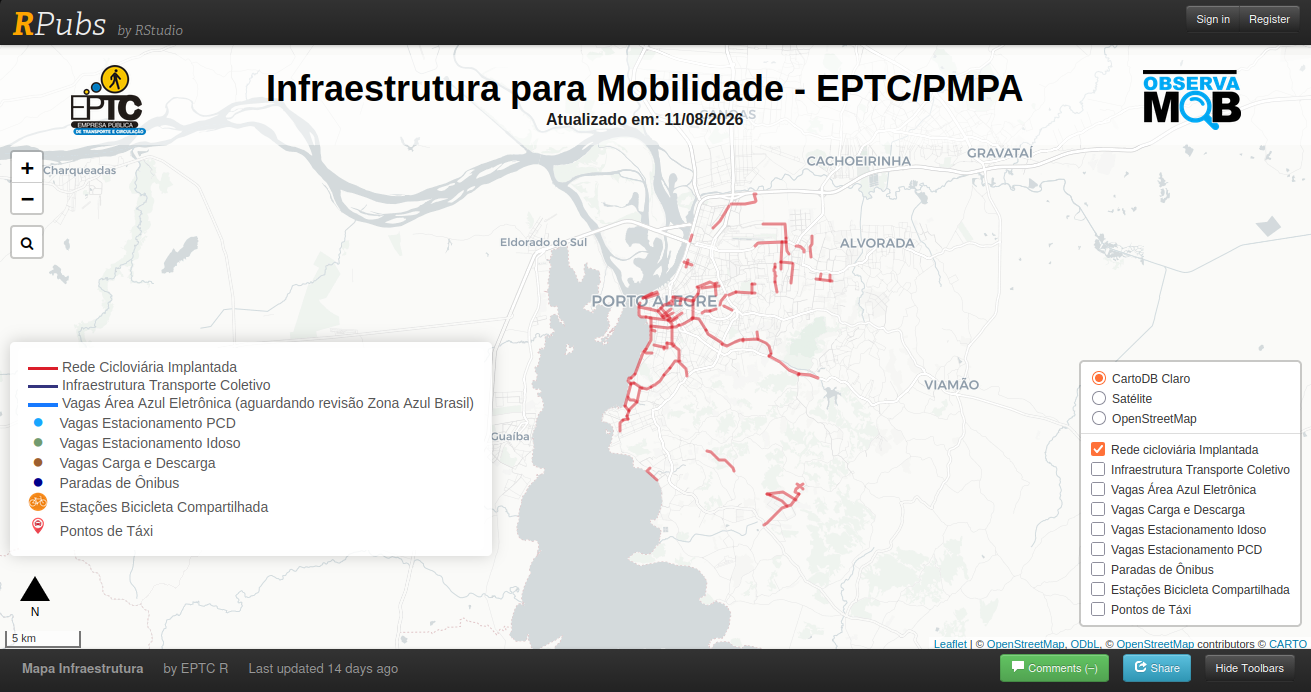
\includegraphics[width=0.9\textwidth]{infra-eptc.png}
    disponível em \url{https://rpubs.com/eptc-r/InfraestruturaMobilidadePOA}
\end{frame}

\begin{frame}{como revolucionar uma cidade com bicicletas}
    \begin{itemize}
        \item \textbf{motivação}: encontrar uma infraestrutura cicloviária eficiente para Porto Alegre sob restrições de custo.
        \item \textbf{modelo matemático}: 
            \begin{itemize}
                \item \alert{vértices} ($V$): interseções de ruas ou pontos de interesse (POIs) da cidade.
                \item \alert{arestas} ($E$): ruas ou ciclovias que conectam os vértices, com pesos representando custos de construção ou manutenção.
                \item \alert{grafo ponderado}: \(G = (V, E, w)\), onde \(w: E \to \mathbb{R}^+\) é a função de peso.
            \end{itemize}
        \item \textbf{objetivo}: aplicar algoritmos de MST para selecionar um subconjunto de arestas que conecte todos os vértices com o menor custo total.
        \item \textbf{metodologia}: usar dados do OpenStreetMap com as bibliotecas \texttt{osmnx} e \texttt{networkx} para construir o grafo da malha cicloviária.
    \end{itemize}
\end{frame}

\begin{frame}{malha primária}
    \begin{itemize}
        \item Rede original: 419 vértices, 566 arestas;
        \item MST: 419 vértices, 418 arestas.
    \end{itemize}
    \centering
    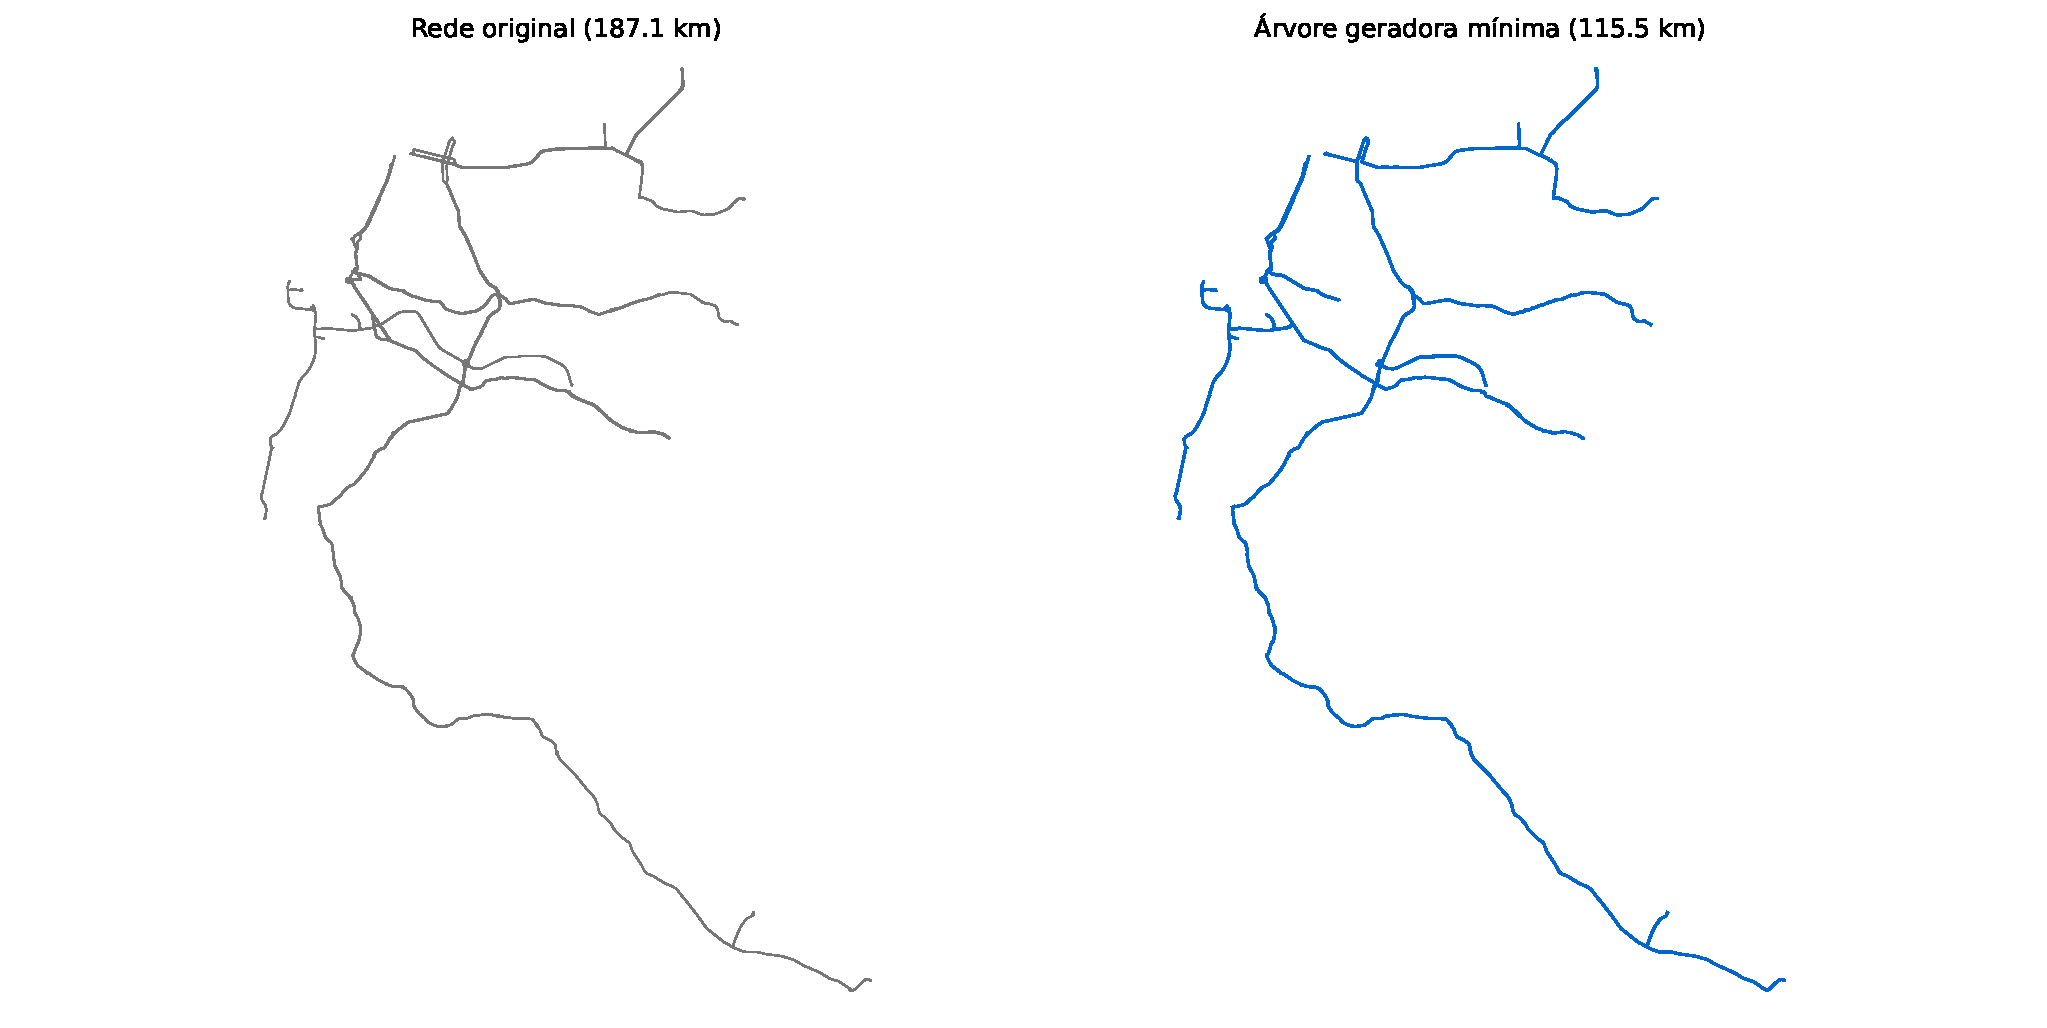
\includegraphics[width=0.9\textwidth]{malha-primaria.pdf}
\end{frame}

\begin{frame}{malha secundária}
    \begin{itemize}
        \item Rede original: 2103 vértices, 3274 arestas;
        \item MST: 2103 vértices, 2102 arestas.
    \end{itemize}
    \centering
    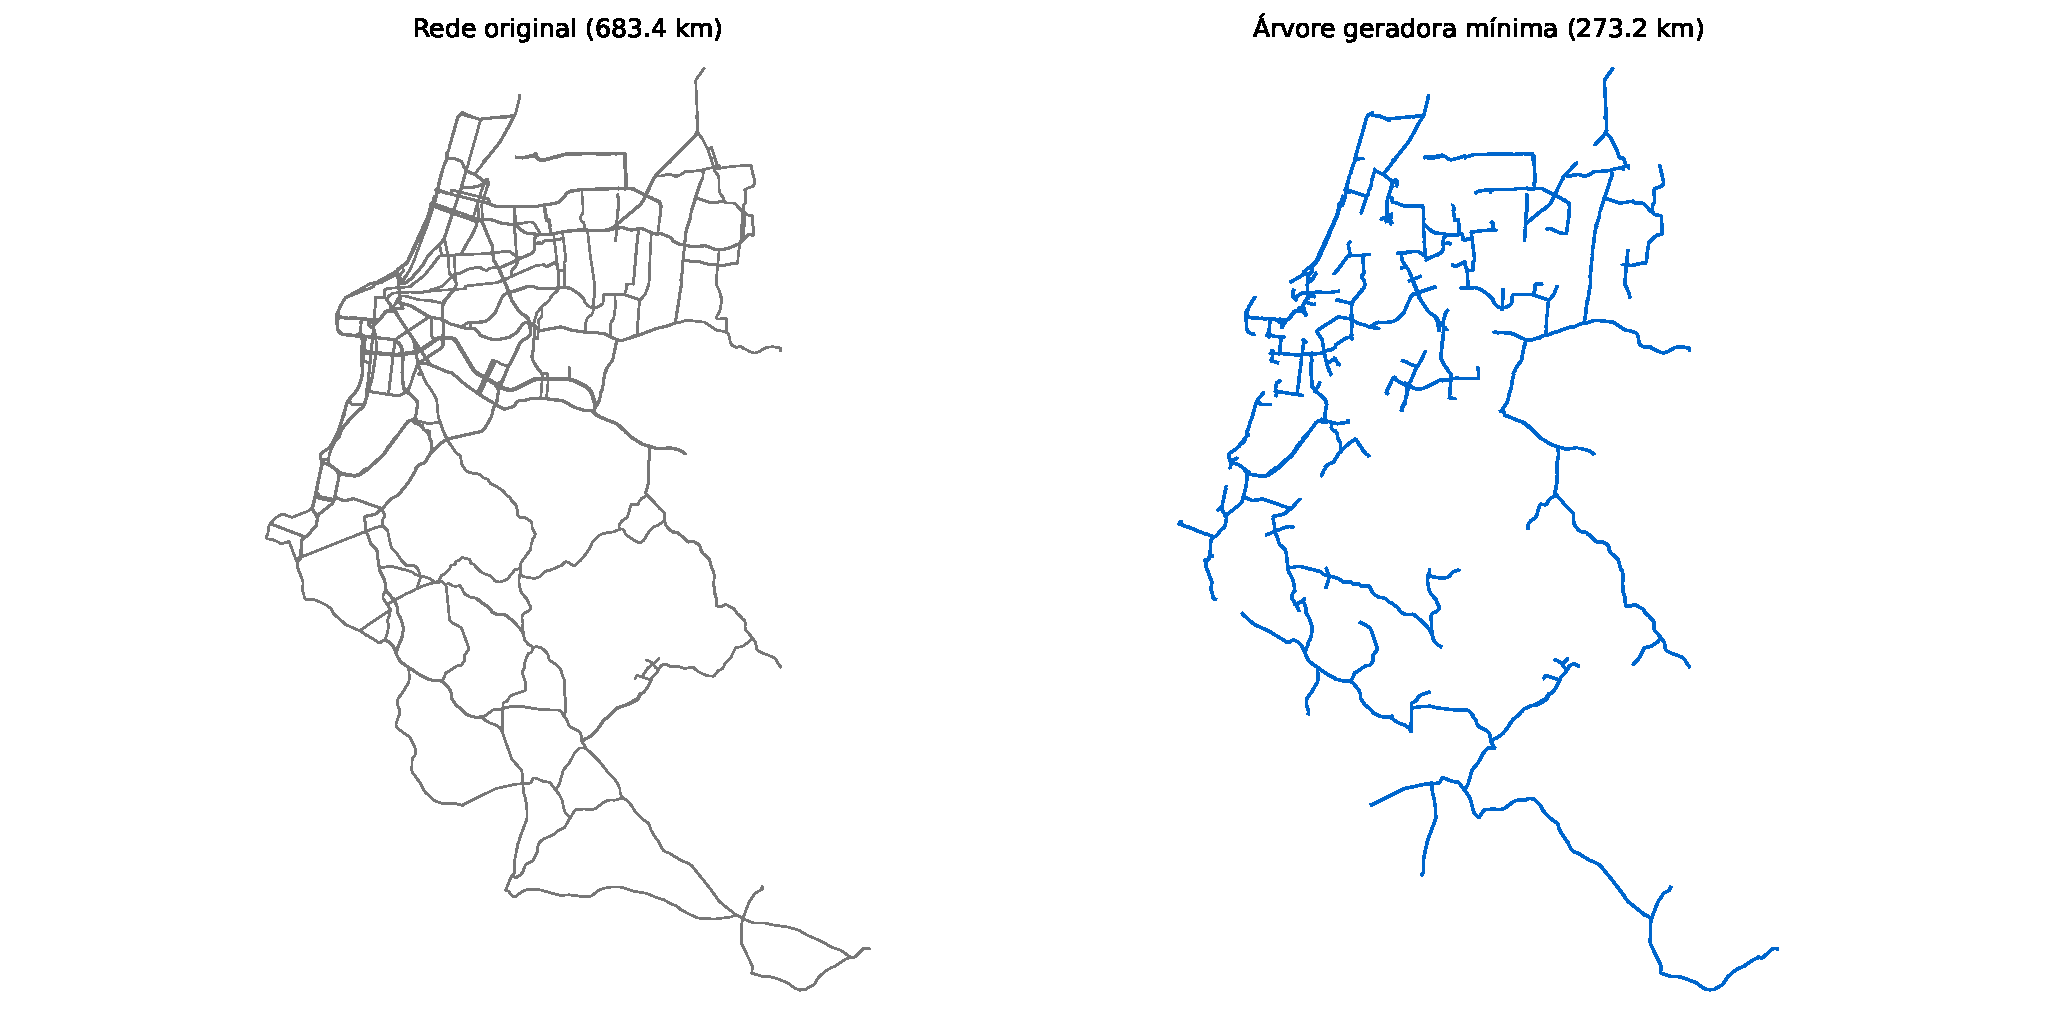
\includegraphics[width=0.9\textwidth]{malha-secundaria.pdf}
\end{frame}

\begin{frame}{malha terciária}
    \begin{itemize}
        \item Rede original: 4523 vértices, 7301 arestas;
        \item MST: 4523 vértices, 4522 arestas.
        \item \emph{obs.:} observa a quilometragem da malha da MST.
    \end{itemize}
    \centering
    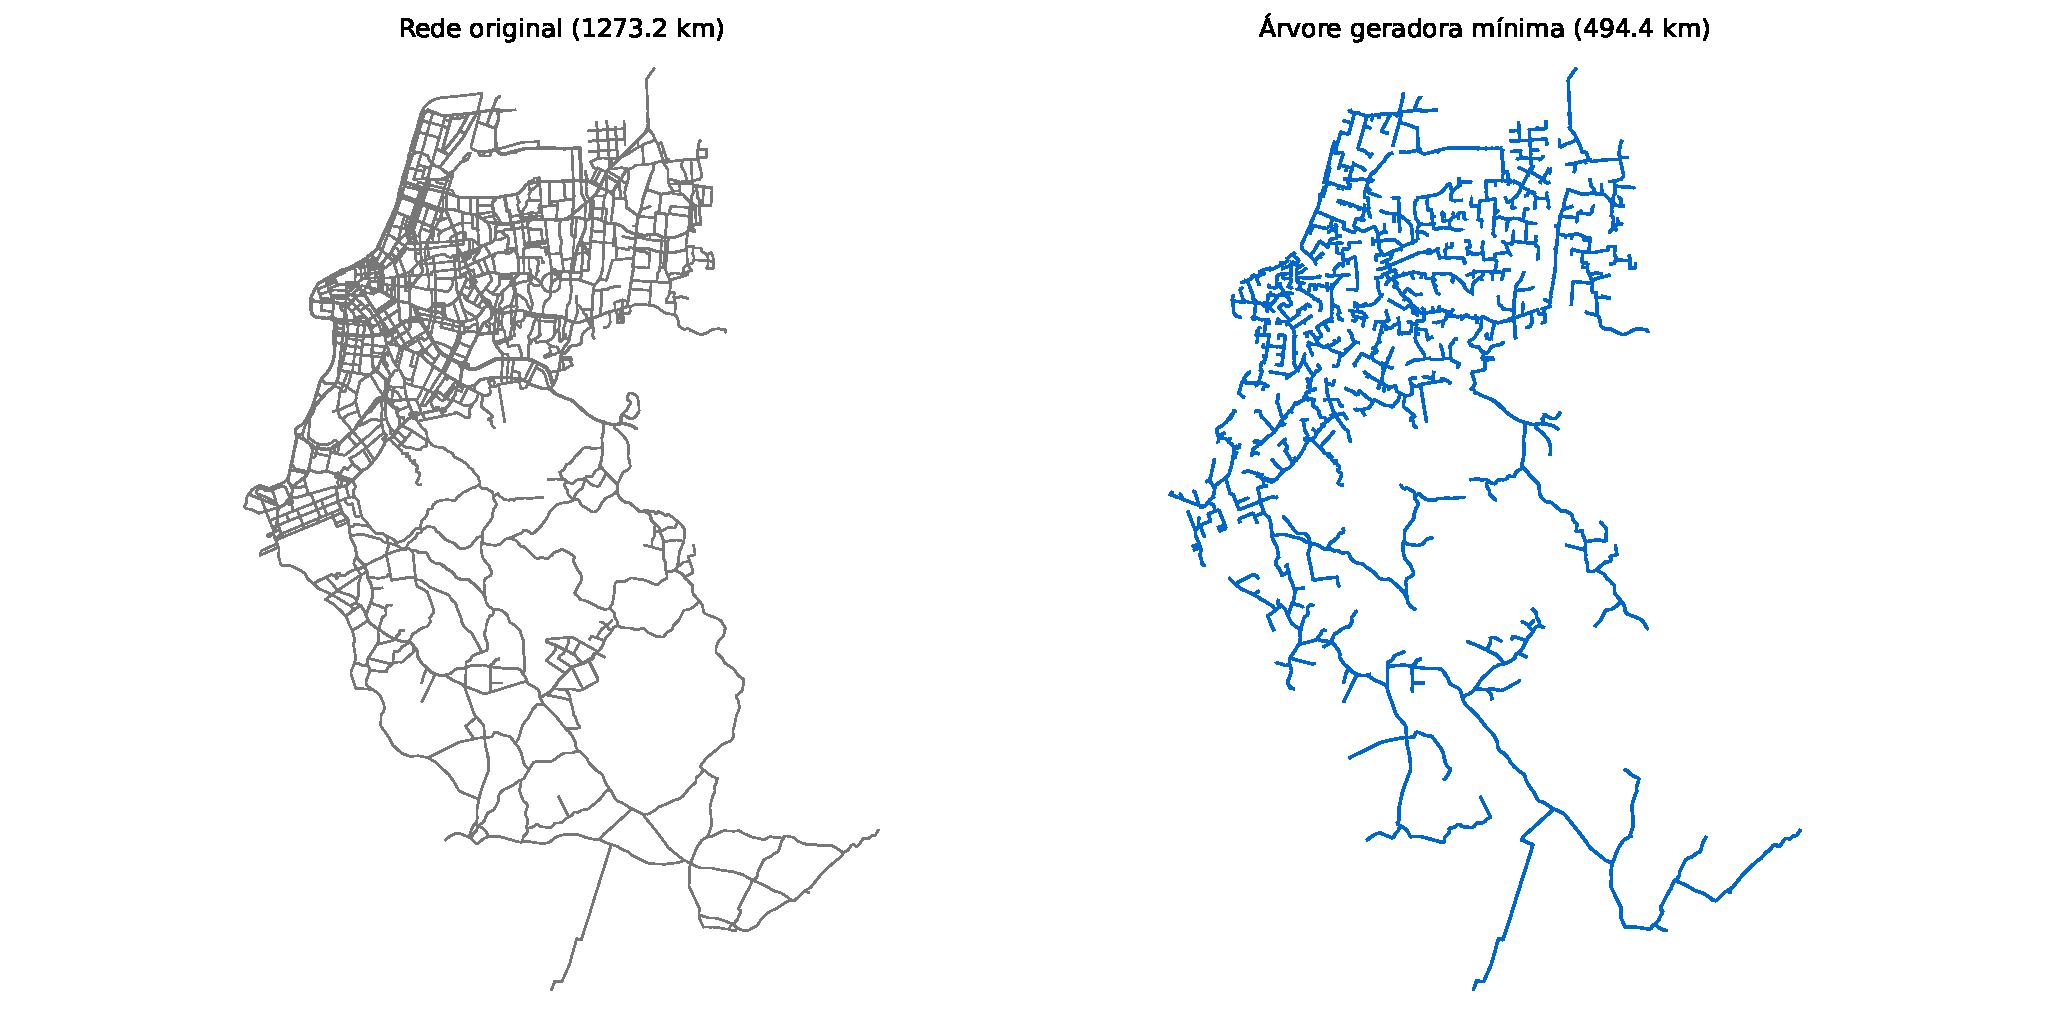
\includegraphics[width=0.9\textwidth]{malha-terciaria.pdf}
\end{frame}

\begin{frame}{árvores fazem sentido?}
    \begin{itemize}
        \item \textbf{QUESTÃO}: as árvores geradoras mínimas (MST) são a melhor abordagem para criar uma malha cicloviária eficiente?
        \item \textbf{PROBLEMAS!!!}
            \begin{itemize}
                \item \emph{a armadilha da topologia da árvore}: a inexistência de ciclos significa que não há rotas alternativas.
                \item \emph{folhas são caras}: o algoritmo força infraestrutura em becos residenciais para satisfazer a conectividade do grafo.
                \item \emph{Porto Alegre tem roça}: a demanda por infraestrutura cicloviária é muito menor em áreas rurais (que são extensas) do que em áreas urbanas.
            \end{itemize}
    \end{itemize}
\end{frame}

\begin{frame}{outras abordagens que não tive tempo para implementar}
    \begin{enumerate}
        \item \textbf{pontos de interesse (POI)}.
            \begin{itemize}
                \item identificar POIs relevantes (escolas, universidades, hospitais, centros comerciais, parques) e priorizar a conectividade entre eles.
                \item usar algoritmos de MST para conectar POIs, mas permitir ciclos em áreas de alta demanda, garantindo rotas alternativas.
            \end{itemize}
        \item \textbf{limitar a extensão por bolas}.
            \begin{itemize}
                \item definir uma distância máxima (raio) a partir de cada POI ou centro urbano, limitando a extensão da malha cicloviária.
                \item aplicar algoritmos de MST dentro dessas regiões delimitadas, evitando a construção de infraestrutura em áreas rurais de baixa demanda.
            \end{itemize}
    \end{enumerate}
\end{frame}

\begin{frame}{mais coisas a se pensar}
    \begin{itemize}
        \item \emph{MST vs. trânsito}: uma MST minimiza o custo de construção, mas redes de trânsito precisam levar em conta o \alert{tempo de viagem} do usuário, que pode não ser minimizado por uma MST.
        \item \emph{$t$-spanner}: usar $t$-spanners para garantir que a distância entre quaisquer dois vértices na malha cicloviária seja no máximo \(t\) vezes a distância mais curta no grafo original, permitindo ciclos e rotas alternativas.
        \item \emph{mais critérios de custo}: incorporar a declividade, velocidade da via, volume de tráfego, etc. como fatores de peso para a construção da malha cicloviária.
    \end{itemize}
\end{frame}

\end{document}